\documentclass[11pt, letterpaper]{article}
%basic packages
\usepackage[utf8]{inputenc}
\usepackage[T1]{fontenc}
\usepackage{graphicx}
\usepackage[margin=1in]{geometry}
\usepackage[usenames,dvipsnames]{xcolor}

%math
\usepackage{amsmath, amsthm, amsfonts, amssymb, mathtools}
\usepackage{mathrsfs}
\usepackage{cancel}
\usepackage{siunitx} %phyjsicsssss
\usepackage{bbm} %mathbb for numbers
\usepackage[all]{xy} % https://texdoc.org/serve/xyguide.pdf/0
\makeatletter
\renewcommand*\env@matrix[1][c]{\hskip -\arraycolsep
  \let\@ifnextchar\new@ifnextchar
  \array{*\c@MaxMatrixCols #1}}
\makeatother %matrix realignment

%misc
\usepackage{float}
\usepackage[hyphens]{url}
%\definecolor{page}{HTML}{242526}
%\pagecolor{page}
\usepackage{booktabs} %the \toprule and \bottomrule thick lines on tables
\usepackage{hyperref}

%my commands
\DeclarePairedDelimiter\bra{\langle}{\rvert} %Bra
\DeclarePairedDelimiter\ket{\lvert}{\rangle} %Ket
\DeclarePairedDelimiterX\braket[2]{\langle}{\rangle}{#1\,\delimsize\vert\,\mathopen{}#2} %Bra-ket
\newcommand{\pvec}[1]{\vec{#1}\mkern2mu\vphantom{#1}} % from https://tex.stackexchange.com/questions/120029/how-to-typeset-a-primed-vector
\newcommand{\hati}{\boldsymbol{\hat{\textbf{\i}}}}
\newcommand{\hatj}{\boldsymbol{\hat{\textbf{\j}}}}
\newcommand{\hatk}{\boldsymbol{\hat{\textbf{k}}}}
\newcommand{\R}{\mathbb{R}}
\DeclareMathOperator{\diag}{diag}
\DeclareMathOperator*{\argmax}{arg\,max}
\DeclareMathOperator*{\argmin}{arg\,min}

%theorems
\usepackage{tikz}
\usepackage{tikz-cd}
\usepackage[framemethod=TikZ]{mdframed}
\usepackage{thmtools}
\newtheorem{theorem}{Theorem}
\newtheorem{corollary}{Corollary}
\newtheorem{lemma}{Lemma}
\newtheorem{proposition}{Proposition}

% slightly neater (imo) theorems
%\declaretheoremstyle[headfont=\bfseries, bodyfont=\normalfont, mdframed={linewidth=1pt, bottomline=false, topline=false, rightline=false, leftline=false}]{theorem}
%\declaretheorem[numbered=yes, style=theorem, name=Theorem]{theorem}
%\declaretheorem[numbered=yes, style=theorem, name=Lemma]{lemma}
%\declaretheorem[numbered=yes, style=theorem, name=Corollary]{corollary}
%\declaretheorem[numbered=yes, style=theorem, name=Proposition]{proposition}

% Side Indented Theorems - https://tex.stackexchange.com/questions/429339/shifting-newtheorem
\newtheoremstyle{side}{}{}{\advance\leftskip3cm\relax\itshape\normalfont}{-4pt}
{\bfseries}{}{0pt}{
\makebox[0pt][r]{
  \smash{\parbox[t]{2.5cm}{\raggedright\thmname{#1}.
  \thmnote{\newline(#3)}}}
  \hspace{10.1pt}}}

\theoremstyle{side}
\newtheorem*{note}{Note}
\newtheorem*{intuition}{Intuition}
\newtheorem*{claim}{Claim}
\newtheorem*{prev}{As Previously Seen}

\theoremstyle{definition}
\newtheorem{definition}{Definition}
\newtheorem*{remark}{Remark}
\newtheorem*{example}{Example}
\newtheorem*{notation}{Notation}

\renewcommand{\qedsymbol}{$\blacksquare$}
\declaretheoremstyle[headfont=\bfseries, bodyfont=\normalfont, mdframed={linewidth=1pt, bottomline=false, topline=false, rightline=false, innertopmargin=0pt, innerbottommargin=0pt}, qed=\qedsymbol]{proof}
\declaretheorem[numbered=no, style=proof, name=Proof]{replacementproof}
\renewenvironment{proof}[1][]{\begin{replacementproof}}{\end{replacementproof}}

%fancy headers
\usepackage{fancyhdr}
\pagestyle{fancy}
\fancyhead{}\fancyfoot{}
\fancyfoot[R]{\thepage}
\fancyfoot[C]{\leftmark}

%lectures, taken from (https://castel.dev/post/lecture-notes-3)
\makeatother
\def\@lecture{}%
\newcommand{\lecture}[3]{%
	\ifthenelse{\isempty{#3}}{%

		\def\@lecture{Lecture #1}%
	}{%
		\def\@lecture{Lecture #1: #3}
	}
	\subsection*{\@lecture}
	\hfill{\small\textsf{#2}}\par
}
\makeatletter
\author{Grant Talbert}

\usepackage{titlepageBU}
\usepackage{qtree}
\title{The Tile Game}
\date{09/19/24}
\courseID{MA 293}
\professor{Dr. Borkovitz}
\courseSection{A1}
\renewcommand{\mod}[1]{\;(\text{mod}\;#1)}
\contributor{Dr. Borkovitz}
\begin{document}
\makereport
\begin{abstract}
	This report analyzes the Tile game. We employ mathematical strategies to identify, and rigorously verify, a method to consistently win this game. In this paper, we employ the method of overusing greek letters to make the math look more complex than it is in reality. I did not really proofread this paper because I'm too tired.

	A brief word on abiding by the assignment guidelines: The description of the winning strategy is outlined in Section 3. The justification is done mathematically through a series of proofs in section 2, then explained conceptually in section 3. The reflection is contained within Section 4. The necessary introduction is contained within Section 1, along with some mathematical background in section 2. Sections 1, 3, and 4 contain many representations to build intuition for the mathematical formalism employed in Section 2. All definitions are clearly made either in Section 2, or in each individual proposition.
\end{abstract}
\section{Background}
\label{sec:1}
The ``Tile Game'' is a two-player game involving the manipulation of a set of tiles according to the following rules:
\begin{itemize}
	\item Players alternate turns.
	\item On their turn, a player can choose to take either one or two tiles.
	\item The player who takes the last tile looses.
\end{itemize}
For example, consider the following game played with 6 tiles.
\begin{enumerate}
	\item Player 1 takes 2 tiles (4 tiles remaining).
	\item Player 2 takes 2 tiles (2 tiles remaining).
	\item Player 1 takes 1 tile (1 tile remaining).
	\item Player 2 takes 1 tile (0 tiles remaining).
\end{enumerate}
Since Player 2 took the last tile, they lose the game.

Due to the simplicity of the game, it makes sense that there is a \emph{solution} to the game; that is, there is a ``correct'' way to play the game that guarentees victory. In the case of our game with 6 initial tiles, there are a small enough number of possible games that we can reasonably create a tree diagram, categorizing every possible game. In \hyperlink{fig:1}{figure 1}, each node indicates either the number of tiles remaining, or if there are no tiles remaining, it indicates the loser of the game.

Players 1 and 2 lose a similar amount of games, specifically 6 and 7, respectively. However, the solutions are arranged in such a way that player 1 can reasonably avoid losing the game. Consider the branch where player 1 begins by taking 2 tiles, leaving 4 tiles in play. If player 2 takes another two tiles, player 1 has the following options:
\begin{itemize}
	\item Take 2 tiles and lose the game, or
	\item Take 1 tile, forcing player 2 to take the last tile and lose.
\end{itemize}
Clearly, player 1 would take a single tile. Player 1 is ``in control of the game'' here.

Alternatively, player 2 could take one tile, leaving 3 on the board. Player 1 now has the following options:
\begin{itemize}
	\item Take 2 tiles, forcing player 2 to take the last tile and lose, or
	\item Take only 1 tile, which allows player 2 to win the game by only taking 1 as well.
\end{itemize}

\Tree[.6 [.5 [.4 [.3  [.2 [.1 [.\textbf{P2}  ]] [.\textbf{P1}  ]][.1 [.\textbf{P1}  ]]][.2 [.1 [.\textbf{P1}  ]] [.\textbf{P2}  ] ] ] [.3 [.2 [.1 [.\textbf{P1}  ]] [.\textbf{P2}  ]][.1 [.\textbf{P2}  ]]]]
	[.4 [.3  [.2 [.1 [.\textbf{P1}  ]] [.\textbf{P2}  ]][.1 [.\textbf{P2}  ]]][.2 [.1 [.\textbf{P2}  ]] [.\textbf{P1} ] ] ]]
\begin{center}
	\noindent Figure 1: Tree Diagram for $\eta =6$\hypertarget{fig:1}{}
\end{center}

Again, player 1 has a forced victory by choosing to take 2 tiles. So no matter what player 2 chooses on their first move, player 1 can force a victory if they take 2 tiles on their first move.

As a corollary of this analysis, we now know that if it's player 1's turn when 4 tiles are on the board, they will lose. We also saw that if it's player 1's turn when 3 tiles are in play, they will also always win. Looking at the other possible starting move for player 1, which is taking 1 tile, we can see that player 2 has the following two options to respond:
\begin{itemize}
	\item Take one tile, leaving 4 tiles on the board for player 1's turn, leading to a victory for player 2, or
	\item Take two tiles, leaving 3 tiles on the board for player 1's turn, leading to a victory for player 1.
\end{itemize}
Player 2 would take two tiles in this case, forcing player 1 to lose the game. However, player 1 can avoid this by simply taking 2 tiles on their first turn, guarenteeing them a win.

From this pre-analysis, we know that when some  specific numbers of tiles are on the board, such as 3 or 5, the player who's move it is can guarentee a victory. However, more importantly, we know that there are specific numbers of tiles, such as 4, where whoever's move it is cannot avoid a defeat, if the game is played optimally. It is the pattern of \emph{losing tiles} that gives rise to the set of \emph{winning tiles}, as the following brief analysis will show.

Consider the following case: there is one tile on the board, and it's your move. You cannot take less than 1 tile, so you must take the final tile, forcing you to lose the game. This is a \emph{losing tile}. It is thus the other player's goal to make it be your turn when only 1 tile remains. If 2 tiles are on the board, they can accomplish this by taking only 1 tile, making the 2nd tile a \emph{winning tile}. Additionally, if 3 tiles are on the board, they can take 2 tiles, and it is your move on 1 tile. This is another winning tile.

Now consider the case of 4 tiles on the board. If you take 1 tile, 3 will remain, and if you take 2, then 2 will remain. Both 2 and 3 are winning tiles, so you have no choice but to make it your opponent's turn on a winning tile. Thus, 4 is another losing tile. And this logic continues recursively; for 5 and 6 tiles, your opponent can take just enough to make it your turn on 4 tiles, but for 7 tiles, they will make it your turn on either 5 or 6, which are winning tiles. This is well-illustrated in \hyperlink{fig:2}{figure 2}.

\begin{center}
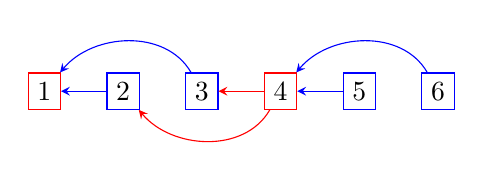
\begin{tikzpicture}
        [->,>=stealth,square/.style={
            draw,
            minimum width=width("#1"),
            minimum height=width("#1")+2*\pgfshapeinnerysep,
            node contents={#1}}]
	\node at (0,0) (1) [square={$1$}, draw = red];
        \node at (1,0) (2) [square={$2$}, draw = blue];
        \node at (2,0) (3) [square={$3$}, draw = blue];
        \node at (3,0) (4) [square={$4$}, draw = red];
        \node at (4,0) (5) [square={$5$}, draw = blue];
        \node at (5,0) (6) [square={$6$}, draw = blue];

	\draw [->,blue] (6) to [out=120,in=50] (4);
	\draw [->,blue] (5) -- (4);
	\draw [->,red] (4) -- (3);
	\draw [->,red] (4) to [out=-120,in=-50] (2);
	\draw [->,blue] (3) to [out=120,in=50] (1);
	\draw [->,blue] (2) -- (1);
    \end{tikzpicture}
    
    \noindent Figure 2: Winning and Losing Tiles for $\eta =6$\hypertarget{fig:2}{}
\end{center}

It is the goal of this paper to mathematically formalize this game, and use this representation to identify and prove the method of guarenteeing a win for any arbitrary number of starting tiles.
\section{Mathematical Reasoning and Solution}
\label{sec:2}

\begin{theorem}[Fundamental theorem of the game]\label{thm:}
	\[
		\forall \eta \in\mathbb{Z}^+\exists \Sigma \subseteq \mathscr{G} (\eta )\backepsilon \exists \rho \in \mathbb{Z}_2 \backepsilon \forall \mathfrak{a} _\mathfrak{k} ,\mathfrak{a} _k = (0,\rho )\land \exists n\in\left\{ 1,2 \right\} \backepsilon\phi _n(\xi ,\rho )\in\mathscr{L} (\eta )
	.\]
	
\end{theorem}

This paper will take a semi-rigorous approach to solving the game. There is more that can be done to formalize the game, but my efforts to do so became highly convoluded, and gave the alternative presentation of \hyperref[lma:1]{theorem 1} as ``\emph{For any $\eta \in\mathbb{Z}^+$, there exists some $\Sigma \subseteq \mathscr{G} (\eta )$ such that there exists some $\rho \in\mathbb{Z}_2$ such that for all $\mathfrak{a} _\mathfrak{k} \in\Sigma $, for all $(\xi ,\rho )\in \mathfrak{a} _\mathfrak{k} $, $\mathfrak{a} _k=(0,\rho ) $ and there exists some $n\in\left\{ 1,2 \right\} $ such that $\left( \Xi \circ \phi _n \right) \left( \xi ,\rho  \right) \in \mathscr{L} (\eta )$.}'' I think it should be apparent why I abandoned this approach.

We begin this section with a brief introduction to some notation used herein, and modular arithmetic. Two integers $a,b\in\mathbb{Z}$ are said to be congruent modulo $n$, notated $a\equiv b\mod{n}$, if and only if there exists some integer $k\in\mathbb{Z}$ such that
\[
	(a-b)=kn
.\]
More simply, if $a$ and $b$ have the same remainder when divided by $n$, then they are congruent modulo $n$. This is the intuitive way to understand it, but the method of showing there exists some $k$ for which the above statement is true will be used in this paper. When such a $k$ exists, we say that $n$ divides $a-b$, notated as $n|(a-b)$. More generally, if $r,s\in\mathbb{Z}$ and there exists some $\lambda \in\mathbb{Z}$ such that (WLOG) $r=\lambda s$, then we say that $s$ divides $r$, and notate it $s|r$.

We continue by standardizing our notation herein. We make use of the method of overusing greek letters in order to make the math look cooler than it is. Since it can often be ambiguous, it should be clarified that we take $0\in\mathbb{N}$ for this paper.
\begin{notation}
	Let $\eta \in\mathbb{Z}^+$ denote the number of starting tiles, and let $\nu_n\in\mathbb{N} $ denote the number of remaining tiles on the $n$th turn, where clearly $n\in\mathbb{Z}^+$.
\end{notation}
We now make the following definition.
\begin{definition}[Losing Tiles]\label{dfn:1}
	Let $\eta \in\mathbb{Z}^+$ denote some starting number of tiles. Then the set of losing tiles for this $\eta $, written as $\mathcal{L} (\eta )$, is given as
	\[
		\mathcal{L} (\eta )\coloneqq \left\{ n\in\mathbb{N} \mid n\leq \eta \land  n\equiv 1\;(\text{mod}\;3) \right\} 
	.\]
	This is the set of all natual numbers $n$ such that both $n\leq \eta $ and $n\equiv 1\;(\text{mod}\;3)$ are true.
\end{definition}
It's important to remark here that although we have called the set $\mathcal{L} (\eta )$ the set of ``losing tiles'', \emph{we have yet to rigorously prove its significance}. This is the purpose of \hyperref[lma:1]{theorem 1}.
\begin{theorem}[Fundamental theorem of the tile game]\label{lma:1}
	Consider a game with starting tiles $\eta \in\mathbb{N}$ and remaining tiles $\nu_n \in\mathbb{N},\nu_n \leq \eta $ on turn number $n$. Suppose $\nu_n \geq 4$. Let it be \textbf{player} \textbf{1}'s turn. If $\nu_n \in \mathcal{L} (\eta )$, then no matter what move player 1 makes, there will exist a possible move for player 2 such that the board after their turn, $\nu_{n+2}$, has $\nu _{n+2}\in \mathcal{L} (\eta )$.
\end{theorem}
\begin{proof}
	There are only two possible moves for player 1 to make:
	\begin{itemize}
		\item Player 1 can take 1 tile, or
		\item Player 1 can take 2 tiles.
	\end{itemize}
	We will consider both cases.

	\textbf{Case 1: Player 1 takes one tile.} Recall that for some $\nu_n\in\mathcal{L} (\eta )$, we must have both $\nu_n \leq \eta $ and $\nu _n \equiv 1\mod{3}$. We will use this second fact to our advantage. Additionally, we know $\nu_n\geq 4$, so by removing 1 tile, we will have $\nu _{n+1}\geq 3$, and thus $\nu _{n+1}\in\mathbb{N}$. Therefore, $\nu _{n+1}$ is a valid board position. Now suppose that player 2 takes two tiles on their next turn. We have $\nu _{n+2}\geq 1$, and thus $\nu _{n+2}\in\mathbb{N}$, so $\nu _{n+2}$ is still a valid board position. Now notice that the total number of tiles that have been taken in these two moves is $2+1=3$, and thus the total remaining number of tiles $\nu _{n+2}$ is given as
	\[
		\nu _{n+2}=\nu -3
	.\]
	It follows that
	\[
		\nu _{n+2}-\nu =-3
	.\]
	We know that for any $a,b\in\mathbb{Z}$, $a\equiv b\mod{3}$ if and only if $3|(a-b)$. Since $\nu _{n+2}-\nu =-3$ and $3|(-3)$ since $-3=(-1)3$, we have
	\[
	\nu _{n+2}\equiv \nu \mod{3}
	.\]
	However, we know $\nu \equiv 1\mod{3}$. Since congruence modulo $n$ is an equivalence relation, by the transitive property of equality we have
	\[
		\nu _{n+2}\equiv 1\mod{3}
	.\]
	We have thus proven that if player 1 takes 1 tile, and player 2 responds by taking 2 tiles, we have $\\nu _{n+2}\equiv 1\mod{3}$, and thus $\nu _{n+2}\in\mathcal{L} (\eta )$. It remains to be shown the same is true for case 2.

	\textbf{Case 2: Player 1 takes two tiles}. The proof of case 2 follows by the same logic as case 1. Player 2 can respond by taking 1 tile, making the total number of tiles taken by player 1's next turn equal to 3. We have $\nu_{n+2}\geq 4-3=1$, and thus $\nu _{n+2}\in\mathbb{N}$ is a valid board position. It also follows that
	\begin{align*}
		&\qquad\,\,\,\, \nu _{n+2}=\nu -3\\
		&\implies \nu _{n+2}-\nu =-3\\
		&\implies \nu _{n+2}\equiv \nu \equiv 1\mod{3}\\
		&\implies \nu _{n+2}\equiv 1\mod{3}
	.\end{align*}
	We thus have $\nu _{n+2}\in\mathcal{L} (\eta )$ if player 2 takes 1 tile.
\end{proof}
We present the following corollary, which encapsulates the significance of \hyperref[lma:1]{theorem 1}.
\begin{corollary}\label{cor:1}
	Let $\eta \in\mathbb{N}$ be the number of starting tiles, and let the number of turns for the $n$th move $\nu_n\in\mathbb{N}$ have $\nu _n\in\mathcal{L} (\eta )$. Suppose it is player 1's turn on move $n$. Then there exists a method by which player 2 will win the game, regardless of what player 1 does. By extension, for $\eta \in \mathcal{L} (\eta )$, there exists a method by which player 2 will always win, and conversely for $\eta \notin \mathcal{L} (\eta )$, there exists a method by which player 1 will always win.
\end{corollary}
\begin{proof}
For convenience, we will use the following notation. Define $\mu_n$ to be the $n$th \textbf{smallest} element of $\mathcal{L} (\eta )$ for an arbitrary $\eta $. So $\mu _1=1$, $\mu_2=4$, and so on, provided $\eta $ is sufficiently large. In other words, $\mu_n = 1+3n$.

	We will use the method of proof by induction to show it to be true that for some board position with tile count $\mu _n\in\mathcal{L} (\eta )$, the player who's move it is can be forced to lose. Without loss of generality, let this player be player 1. The smallest element of $\mathcal{L} (\eta )$ for any $\eta \geq 1$ is $1$. For $\mu_1 =1$, player 1 has only the option to take one tile. When they take the tile, there will be no tiles remaining, and player 2 will win.

	Now suppose player 1 will lose if it is their turn for $\mu _n\in \mathcal{L} (\eta )$. We must show for the next greatest element of $\mathcal{L} (\eta )$, herein $\mu_{n+1} $, if it is again player 1's turn, they will lose. We know already that $\mu _{n+1}\in \mathcal{L} (\eta )$. By \hyperref[lma:1]{theorem 1}, we know that no matter what player 1 does, there exists a way for player 2 to make their next move have tile count $\mu_{n+1}-3\in\mathcal{L} (\eta )$. By definition, $\mu_{n+1}-3=\mu_n$. We know already that there exists a way for player 2 to force a win from this board position, and thus there exists a way for player 2 to force a win from board position $\mu_{n+1}$. Therefore, for board position $\nu_n\in\mathcal{L} (\eta )$, there exists a way for the player who is not moving to force a win.

	From this, it follows immediately that for $\eta \in \mathcal{L} (\eta )$, player 2 can force a win, and for $\eta \notin \mathcal{L} (\eta )$, there exists a way for player 1 to force a win.
\end{proof}
\section{Significance and Explanation}
\label{sec:3}
Since all the mathematical jargon can be difficult to understand, we present a thorough explanation of \hyperref[lma:1]{theorem 1} and \hyperref[cor:1]{corollary 1}. If we recall from \hyperref[sec:1]{section 1}, we had a notion of a ``losing tile''. For some quantities of tiles, it's possible to guarentee the player who moved when that many tiles were in play would lose, if the other player plays optimally. The way this worked was by creating a chain of losing tiles. Clearly, 1 is a losing tile, since you have to take the tile and then lose the game. However, as illustrated in \hyperref[fig:2]{figure 2}, 4 is also a losing tile, since if it's your turn on 4 tiles, there's a way the other player can also force it to be your turn on 1 tile. If you take 1 tile, they take 2, and if you take 2, they take 1. The key thing to notice here is that in these two turns, there are always exactly 3 tiles taken in total.

This can be generalized. In \hyperref[fig:3]{figure 3}, we extend \hyperref[fig:2]{figure 2} to include a few more tiles.

\begin{center}
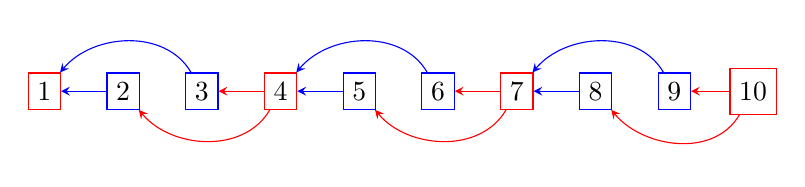
\begin{tikzpicture}
        [->,>=stealth,square/.style={
            draw,
            minimum width=width("#1"),
            minimum height=width("#1")+2*\pgfshapeinnerysep,
            node contents={#1}}]
	\node at (0,0) (1) [square={$1$}, draw = red];
        \node at (1,0) (2) [square={$2$}, draw = blue];
        \node at (2,0) (3) [square={$3$}, draw = blue];
        \node at (3,0) (4) [square={$4$}, draw = red];
        \node at (4,0) (5) [square={$5$}, draw = blue];
        \node at (5,0) (6) [square={$6$}, draw = blue];
	\node at (6,0) (7) [square={$7$}, draw = red];
	\node at (7,0) (8) [square={$8$}, draw = blue];
	\node at (8,0) (9) [square={$9$}, draw = blue];
	\node at (9,0) (10) [square={$10$}, draw = red];


	\draw [->,red] (10) to [out=-120,in=-50] (8);
	\draw [->,red] (10) -- (9);
	\draw [->,blue] (9) to [out=120,in=50] (7);
	\draw [->,blue] (8) -- (7);
	\draw [->,red] (7) -- (6);
	\draw [->,red] (7) to [out=-120,in=-50] (5);
	\draw [->,blue] (6) to [out=120,in=50] (4);
	\draw [->,blue] (5) -- (4);
	\draw [->,red] (4) -- (3);
	\draw [->,red] (4) to [out=-120,in=-50] (2);
	\draw [->,blue] (3) to [out=120,in=50] (1);
	\draw [->,blue] (2) -- (1);
    \end{tikzpicture}
    
    \noindent Figure 3: Winning and Losing Tiles for $\eta =10$\label{fig:3}
\end{center}

The key thing to notice here is that starting with the first tile, every third tile is a losing tile, since no matter what you play, the opponent can play a move to make the total tiles taken exactly 3. So every 3rd tile is congruent - not only does the winning/losing status the same for every 3rd tile, but so is the optimal move to play, assuming the tiles in question are winning tiles. The question here is ``does this generalize to an arbitrary number of starting tiles?''

Proving this is the goal of \hyperref[lma:1]{theorem 1}. Our hypothesis is that every 3rd tile, starting with the 1st tile, is a losing tile, and that these tiles are losing because the other player can force a chain of losing tiles, terminating at the last tile. This definition is formalized as $\mathcal{L} (\eta )$. This is the set of all integers equivalent to 1 modulo 3 that are less than or equal to $\eta $, the starting number of tiles. If a tile is in this sequence of ``3rd tiles starting with 1'', it will obviously be the $3n+1$th tile for an arbitrary $n\in\mathbb{Z}$, and thus equivalent to 1 mod $3$.  Once we have this formal notion of losing tiles, we can attempt to prove our hypothesis.

In order to prove our hypothesis, we need to show that a chain of losing tiles can be forced. In other words, we need to prove that if player 1 moves when a board position is a losing move - that is, $\nu_n \in \mathcal{L} (\eta )$ for starting position $\eta $ and board position $\nu_n $ - then player 2 has a way to force player 1's next move to \emph{also be a losing move}. So we start with the knowledge that player 1's board position $\nu _n$ is equivalent to 1 modulo 3. We prove this on a case by case basis, but the logic is the same. If player 1 takess 1 tile, we say player 2 takes 2 tiles, and vice versa. The total number of tiles taken is the same, so the logic for both cases is the same after this point. The number of remaining tiles, $\nu _{n+2}$, is simply the board position we started the proof with, $\nu _n$, minus 3 tiles. Thus, $\nu _{n+2}=\nu -3$. The $-3$ is clearly a multiple of 3, and thus if $\nu $ is equivalent to 1 modulo 3, then so must be $\nu _{n+2}$. The rest of the proof is showing this formally, with the logic we gave in the beginning of \hyperref[sec:2]{section 2}. Thus, we formally show that no matter what player 1 does, player 2 will able to force player 1 to move on another losing tile. We are not quite done yet, but our hypothesis appears to be proven.

Before moving on, there is one more curiosity of \hyperref[lma:1]{theorem 1} that should be addressed. We supposed that $\nu_n \geq 4$. The reason for doing this is to ensure a valid board position, since if we have $\nu_n <4$ being a losing position, then $\nu _n$ must equal 1, and then we cannot take 2 tiles, since that would be an invalid board position as $\nu _{n+1}=-1\notin \mathbb{N}$. This is partially why we are not done, as we need to generalize our logic to the 1st tile, but also to an arbitrarily high number of tiles, for $\eta $ sufficiently large.

This generalization is the purpose of \hyperref[cor:1]{corollary 1}. We need to rigorously show that this fact that one losing tile leads to another \emph{actually implies} that the player who moves will lose. We do this with the method of induction, which rather cleanly addresses our case of $\nu _n = 1$. We begin by proving that for $\nu_n = 1$, the player who moves will lose. This proof comes by the definition of the game, and is trivial. Since we do not rely on \hyperref[lma:1]{theorem 1} for this result, taking $\nu _n \geq 4$ is not a factor here. We then show that if we know an arbitrary number of losing tiles (notated $\mu_n$) will lead to a loss, then the \emph{next highest number of losing tiles} (notated $\mu _{n+1}$) will also lead to a loss. In essence, we are showing that if we know we can get one losing position to lose, then this implies the next highest losing position will also lose. And since we have already proven this for 1 tile, and all other losing positions are subject to \hyperref[lma:1]{theorem 1}, we can use that result in the proof. So we simply have if one position is losing, and the next highest position can be played in such a way that yields our position that is known to lose, then that position must also lose. And thus, by the method of induction, we prove the result for an arbitrary $\nu_n$ given $\eta $ sufficiently large. Deciding the optimal first player to move follows immediately, is rather trivial, and is also addressed in the proof.

Thus, we have rigorously proven that for $\eta \equiv 1\mod{3}$, the winning strategy is to go second and take the opposite of your opponent, and for $\eta \not\equiv1\mod{3} $, the winning strategy is to go 1st, take however many tiles are required to make the total number equivalent to 1 modulo 3, then continute taking the opposite of what your opponent takes.


\section{Reflection}
\label{sec:4}
There were two extremely impactful realizations made when solving this problem, one of which has given rise to a visualization used multiple times herein. This first realization came from noticing a pattern by generalizing the number of possible moves we could do. For simplicity, let $\phi _n$ denote a move wherein $n$ tiles are taken, and let $\Phi $ denote the set of all considered moves. Our original game considers $\Phi =\left\{ \phi _1,\phi _2 \right\} $, but considering sets such as $\Phi =\left\{ \phi _1,\phi _2,\phi _3 \right\} $ and $\Phi =\left\{ \phi _1,\ldots,\phi _4 \right\} $ gives rise to an interesting pattern. Herein, we used equivalence modulo 3 extensively. But the significance of the number 3 comes from the fact that if you take the smallest number of tiles you can (1), then the maximum number of tiles that can be taken over your move and your opponent's next move is 3, since $2+1=3$. Changing $\Phi $ changes this maximum number, and keeping this structure $\Phi =\left\{ \phi _1, \dots, \phi _n  \right\} $ gives us equivalence modulo $n+1$ as our relevant relationship. We only realized this pattern after testing multiple sets $\Phi $, however, yet this pattern gave insight into the original tile game by revealing equivalence modulo 3 as the relevant relationship to consider.

The next important insight came from a visualization introduced by Dr. Borkovitz. If we arrange the tiles as shown in \hyperref[fig:4]{figure 4}, the aforementioned relationship becomes obvious.

\begin{center}
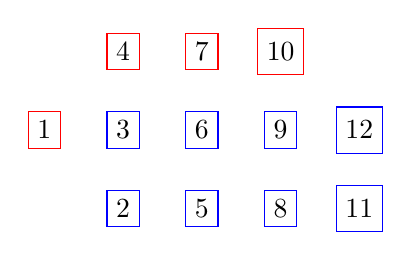
\begin{tikzpicture}
        [->,>=stealth,square/.style={
            draw,
            minimum width=width("#1"),
            minimum height=width("#1")+2*\pgfshapeinnerysep,
            node contents={#1}}]
	\node at (0,1) (1) [square={$1$}, draw = red];
        \node at (1,0) (2) [square={$2$}, draw = blue];
        \node at (1,1) (3) [square={$3$}, draw = blue];
        \node at (1,2) (4) [square={$4$}, draw = red];
        \node at (2,0) (5) [square={$5$}, draw = blue];
        \node at (2,1) (6) [square={$6$}, draw = blue];
	\node at (2,2) (7) [square={$7$}, draw = red];
	\node at (3,0) (8) [square={$8$}, draw = blue];
	\node at (3,1) (9) [square={$9$}, draw = blue];
	\node at (3,2) (10) [square={$10$}, draw = red];
	\node at (4,0) (11) [square={$11$}, draw = blue];
	\node at (4,1) (12) [square={$12$}, draw = blue];
    \end{tikzpicture}
    
    \noindent Figure 4: Tile Layout for $\eta =12$\label{fig:4}
\end{center}

Whoever goes first will take 2 tiles, as we have seen previously. After this, no matter what the second player does, the first player can ``complete the column'' by taking all remaining tiles in the column. Then the players move on to the next column, and the next, until there are no columns remaining. Then, player 2 is forced to take the last tile, securing the victory for player 1. This helped solidify equivalence modulo 3 as the method by which this game could be formalized, and the given strategy could be rigorously shown to be optimal.

For some reason, I'm supposed to talk about my feelings while working on this problem. My feelings when working on math are always one of the following three:
\begin{itemize}
	\item Confusion, usually when first starting a problem or hitting a wall.
	\item Frantic energy, usually whenever I have a good idea. This generally involves running between as many whiteboards as possible and writing as fast as possible.
	\item Satisfaction, usually after finishing a proof or writing something that makes me look way smarter than I actually am.
\end{itemize}
I felt all three of these emotions at the appropriate times during this assignment.

Since I already know about modular arithmetic, my learning edge for this assignment was mostly just writing as good of a writeup as I could, but also figuring out how to apply my knowledge to a problem I had not previously seen, which involves recognizing the proper mathematical knowledge to apply. This is the hardest part for me at this point, as recognizing what methods to apply is not always straightforwards.
\section{Acknowledgements}
Dr. Borkovitz contributed a visualization discussed in \hyperref[sec:4]{section 4}.

\textbf{Academic Integrity -- Please type your name to acknowledge that if you collaborated on this problem, then it was only with classmates from either section of CAS MA 293 (except to have a partner for the game), that you only used allowable resources (notes from class, no Internet searches or AI, etc.), and that you wrote this paper by yourself:}\\
Grant Talbert
\end{document}
